\chapter{Felhasználói dokumentáció} % User guide
\label{ch:user}

\section{Rendszerkövetelmények}

Az alkalmazás csak Ubuntu LTS 20.04 LTS operációs rendszer mellett lett tesztelve, de várhatóan más Linux rendszerek mellett is működőképes. A pontos hardverigény nem lett kimérve, de egy átlagos képességű (egyéb célokra jól használható) számítógépen várhatóan futni fog.

A program futtatásához szükséges, hogy a \textit{pgrep} program telepítve legyen, és a \textit{pgrep} futtatható állomány helye hozzá legyen adva a \textit{PATH}-hoz. Ez Ubuntu 20.04 LTS operációs rendszer esetén alapértelmezett.

\section{Telepítés és indítás}

A program fordításához az alábbiakra van szükség:
\begin{compactenum}
	\item GHC, legalább 8.6.5 verzió (valószínűleg korábbiakra is működik)
	\item Haskell csomagok: \textit{base, cereal \cite{cereal}, fgl \cite{fgl}, ghcid \cite{ghcid}, gtk2hs \cite{gtk2hs}, microlens-platform \cite{microlens}, parsec \cite{parsec}, split \cite{split}, unliftio \cite{unliftio}}, illetve ezen csomagok függőségei. 
\end{compactenum}

A fentiek megléte esetén a program az alábbi paranccsal fordítható: 

\textit{ghc Main.hs -o insertNameHere}

\textit{insertNameHere} helyére írható a futtatható állomány kívánt neve. Az alkalmazás az így kapott futtatható állomány futtatásával indítható el. Fontos, hogy az \textit{Empty.hs} fájl a futtatható állománnyal egy mappában helyezkedjék el, hogy a kiértékelés az ezen dokumentációban leírt módon működjék.

\section{A felhasználói felület áttekintése}

\begin{figure}[H]
	\centering
	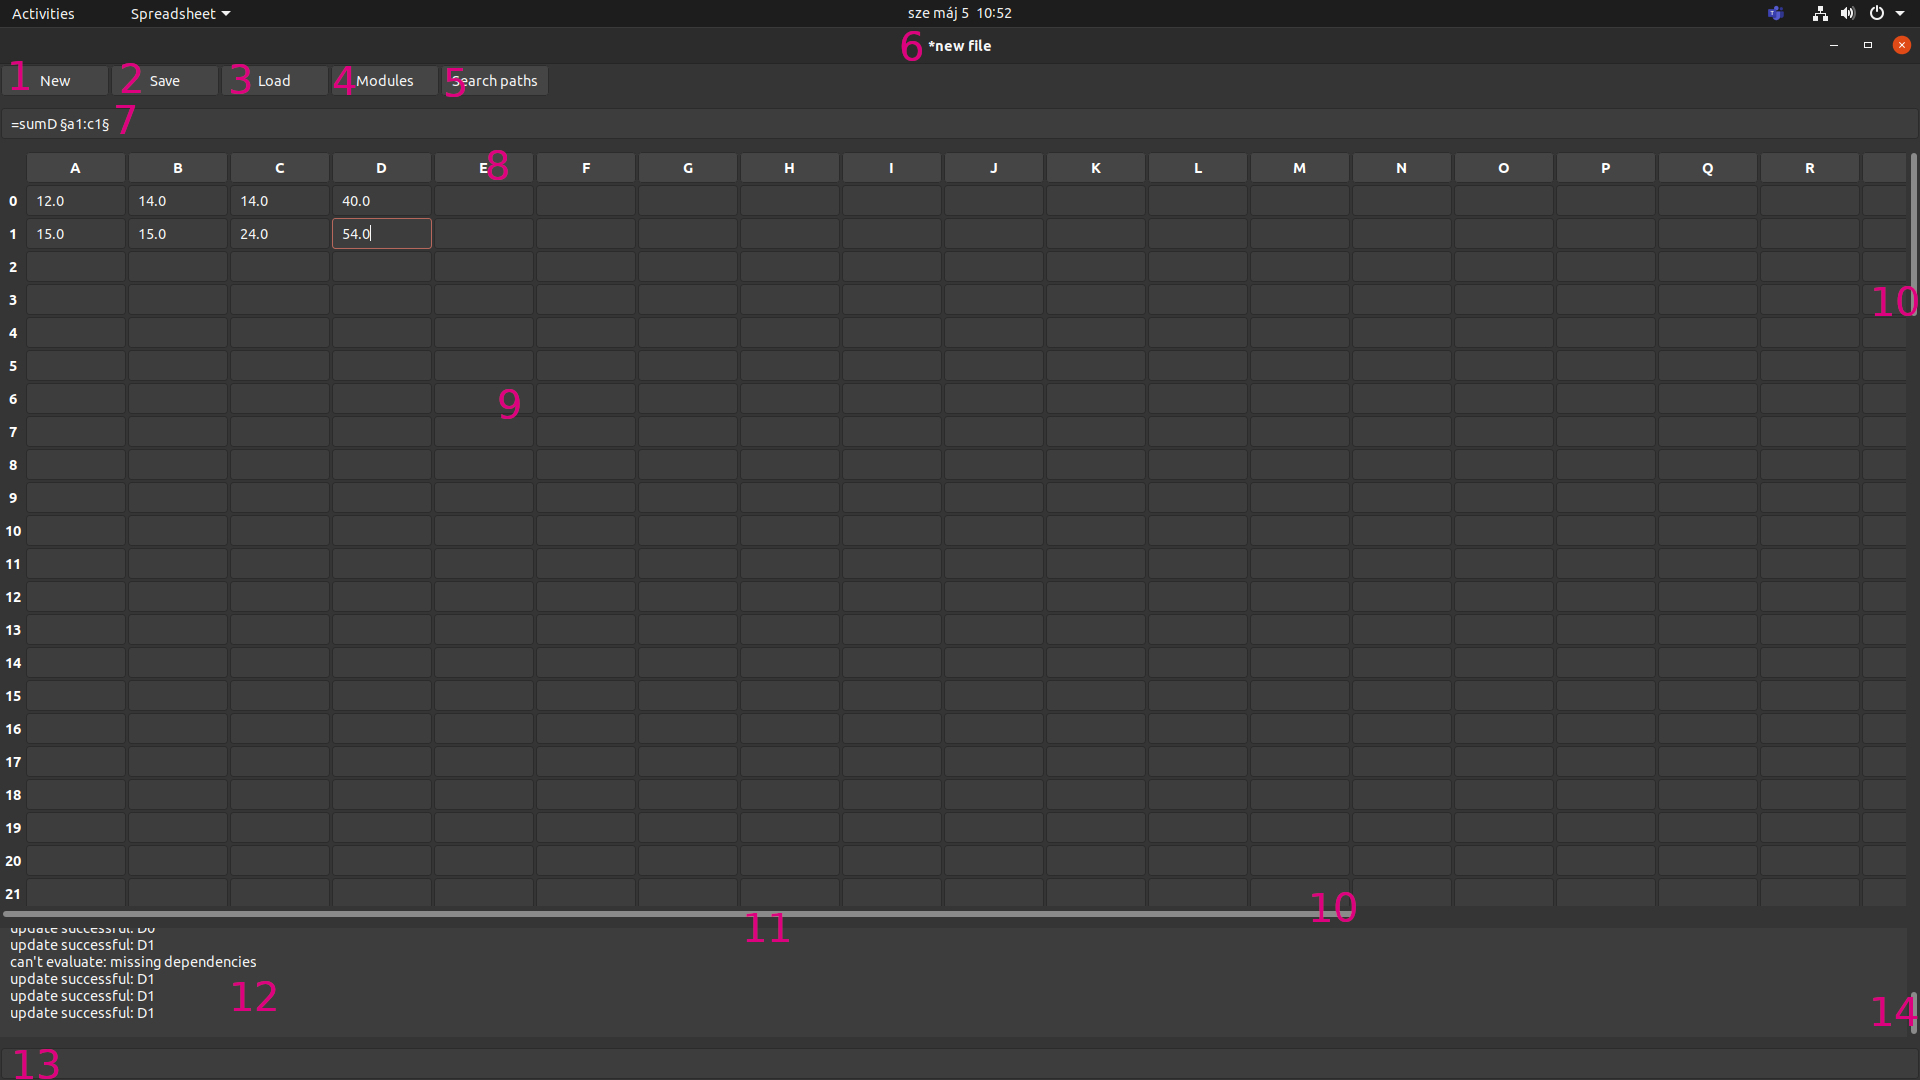
\includegraphics[width=\textwidth]{gui}
	\caption{A felhasználói felület}
	\label{fig:gui}
\end{figure}

\begin{compactenum}
	\item Ezzel a gombbal lehet új számolótáblát létrehozni. Ekkor a számolótábla üres lesz. Billentyűkombináció: Alt-N.
	\item Ezzel a gombbal lehet elmenteni a számolótábla aktuális állapotát. A fájl az alkalmazás saját \textit{.fsandor} kiterjesztésében kerül mentésre. Ha a tábla még nem volt mentve, felugrik egy dialógus, ahol meg lehet adni a mentés útvonalát. Ha már be van töltve egy fájl, a mentés frissíti a mentett fájl tartalmát. Billentyűkombináció: Alt-S.
	\item Ezzel a gombbal lehet fájlt betölteni. Billentyűkombináció: Alt-L.
	\item Ezzel a menüponttal lehet beállítani a háttérben futó GHCi-be betöltendő modulok listáját. A felugró szövegmező minden sora egy modult jelent.
	\item Ezzel a menüponttal lehet beállítani, hogy az alapértelmezett útvonalakon kívül hol keresse a GHCi a betöltendő modulokat. Minden sor egy elérési útvonalat jelent. Az elérési útvonal lehet abszolút (ez utóbbi a javasolt) vagy relatív a futtatható állomány helyéhez képest.
	\item A betöltött fájl neve. Ha épp nincs elmentve a számolótábla, a "*new file" szöveg jelenik meg. Ha a betöltött fájl neve előtt szerepel egy "*", az azt jelenti, hogy a legutóbbi mentés óta történt módosítás.
	\item Kódszerkesztő. Ebbe a sorba lehet kódot írni az aktuálisan kijelölt cellához. A kijelölt cella az a cella, amelyre a felhasználó legutóbb kattintott. A beírt kód akkor kerül kiértékelésre, ha a felhasználó egy másik elemre kattint vagy leüti az entert.
	\item Az oszlop tetején levő gombra kattintva lehetséges beállítani az oszlop karakterekben megadott szélességét. Az oszlopok legfeljebb 100 karakter szélesek lehetnek. Megjegyzés: az átméretezés végrehajtása jelenleg meglehetősen lassú, akár 10 másodpercet is igénybe vehet.
	\item A számolótábla. A számolótábla mérete fixen 26 oszlop és 100 sor. A cellába beírt kód akkor kerül kiértékelésre, ha a felhasználó egy másik elemre kattint vagy leüti az entert.
	\item A számolótábla alján és jobb oldalán található görgőkkel lehet görgetni a számolótáblában.
	\item A számolótábla és a log ablak relatív mérete húzással állítható. 
	\item A log mutatja a végrehajtott akciók (pl. cella kódjának átírása, GHCi query eredménye) eredményét. Jobb oldalt görgethető.
	\item Az alkalmazáshoz tartozó parancssor. A beírt parancs akkor kerül kiértékelésre, ha a felhasználó leüti az entert.
	\item A log üzenetek között a log ablak jobb oldalán található görgővel lehet görgetni.
\end{compactenum}

A kódszerkesztőben, a cellákban és a parancssorban használhatók a megszokott billentyűkombinációk a beírt szöveg manipulálására. (Pl. Ctrl-C, Ctrl-V, Ctrl-X, Ctrl-A)

Az alkalmazás egyelőre nem támogatja számformátum beállítását, ennek megfelelően a belső reprezentáció által biztosított maximális számú tizedesjegy jelenik meg a számokat tartalmazó cellákban.

\section{Cellák és kiértékelés}

\subsection{A kifejezések}

Egy cella tartalma négyféle lehet: üres cella, szám, szöveg vagy formula. A cellába beírt kifejezés pontosan akkor formula, ha az első (nem szóköz) karaktere "=". Amennyiben az első (nem szóköz) karakter nem "=", és a beírt szöveg értelmezhető tizedestörtként, úgy a cella tartalma számként kerül értelmezésre. Minden más esetben a cella tartalma egy string. Példák:
\begin{compactenum}
	\item Szám: "0.12", "-11", "-12.", ".123"
	\item Formula: " =sum [1..10]", "= §\$a\$0§+sumD §a2:b4§"
	\item String: "alma", ".12aa"
\end{compactenum}

A formulákba lehetséges cellahivatkozásokat írni. Kétféle cellahivatkozás létezik:
\begin{compactenum}
	\item Egyszerű hivatkozás. Pl: §a0§,§B\$1§, §\$c\$20§, §\$B10§
	\item Listahivatkozás. Pl: §a0:B4§, §c\$2:c\$10§, §\$a0:b\$10§
\end{compactenum}

A cellahivatkozások nem kisbetű-nagybetű érzékenyek.

A hivatkozásokban található \textit{\$} karakter minden hivatkozás (listahivatkozás esetén mindkét határ) oszlop- és sorneve elé is beszúrható. A \textit{\$} jelnek cellák másolásakor és mozgatásakor van szerepe (részletesebben lásd 2.6.2).

A formula összes többi (nem hivatkozás) része Haskell kódként kerül értelmezésre. A kifejezés Haskell szintaxisnak megfelelése és a típushelyesség a kiértékelés során ellenőriztetik.

Megjegyzés: A cellákba csak numerikus és szöveges adat írható és számítható. Amennyiben a megadott formula más típusú, úgy \textit{Show} példánnyal rendelkező típusok esetén az érték \textit{String} reprezentációja lesz a számítás eredménye, ellenkező esetben pedig hiba lép fel. Pl. az "=[1..5]" formula az "[1,2,3,4,5]" string-re értékelődik ki, az "=\textbackslash x -> x" kifejezés eredménye hiba.

\subsection{A futásidejű reprezentáció}

Egy cella futásidejű reprezentációja egy \textit{Maybe a} típusú érték. Az üres cella reprezentációja \textit{Nothing}, a nemüres cella reprezentációja \textit{Just val}, ahol \textit{val} a cella értéke. A kiszámított értékek is mindig Just-ba csomagoltatnak, hogy a GHCi továbbszámolhasson velük. A valamely cella megváltozásának hatására kezdődő kiértékelési folyamat végrehajtása után az értékek visszaolvasásakor ez a háttérben egy \textit{fromJust} hívással kicsomagolódik, az értékek a cellákban Just nélkül jelennek meg.
Egész szám esetén a kódgeneráló algoritmus figyel arra, hogy olyan literált generáljon a cellaértékből, ami értelmezhető egész típusúként (azaz ilyenkor levágja a tizedesrészt).

A cellahivatkozások feloldását példákon keresztül mutatjuk be. Bal oldalt található a hivatkozás, jobb oldalt a generált kód.
\begin{compactenum}
	\item \textit{§a0§} $\rightarrow$ \textit{fromJust v0}
	\item §a0:a3§ $\rightarrow$ \textit{[v0,v2,v5,v10]}
	\item \textit{§a1:b0§} $\rightarrow$ \textit{[]}
\end{compactenum}

A cellahivatkozások feloldásakor a cellákhoz egy $\mathbb{N} \times \mathbb{N} \rightarrow \mathbb{N}$ bijekción keresztül egy azonosító kerül hozzárendelésre (innen származnak a kódban írt \textit{vi} változónevek. A függvény definíciója megtalálható a fejlesztői dokumentációban (3.2.4). Listahivatkozás feloldásakor a hivatkozott téglalap elemei fentről lefelé és balról jobbra haladva, sorfolytonosan kerülnek a listába. Pl: §a2:c3§ esetén a lista elemeinek sorrendje: [a2,a3,b2,b3,c2,c3]

A relatív és abszolút hivatkozások feloldása között nincs különbség. A kétféle hivatkozástípus közötti különbség csak másoláskor és mozgatáskor jelentkezik.

A fentiek alapján \textit{a} típusú cellára mutató egyszerű hivatkozás ugyanúgy használható, mint egy \textit{a} típusú érték. Az üres cellára való egyszerű hivatkozás hibát okoz. Példák (beírt kód és generált kód):
\begin{compactenum}
	\item A0 kódja: \textit{"12.0"}, B1 kódja: \textit{"=§a0§+11"} $\rightarrow$ B1 értékét kiszámító Haskell kód: \textit{v3 = Just \$ fromJust (Just 12) + 11}
	\item A0 kódja : \textit{""} B1 kódja: \textit{"=§a0§+11"} $\rightarrow$ B1 értékét kiszámító (hibát eredményező) Haskell kód: \textit{v3 = Just \$ fromJust Nothing + 11}
\end{compactenum}

A listahivatkozások feloldásakor azonban a lista elemei \textit{Maybe a} típusúak maradnak. Példa:

A0 kódja: \textit{"12"}, A1 kódja: \textit{"13"}, A2 kódja: \textit{=sum §a0:a1§} $\rightarrow$ A2 értékét kiszámító (típushibás) Haskell kód: \textit{v5 = Just \$ sum [Just 12, Just 13]}

Ez látszólag komoly problémákat eredményez, de a standard könyvtár (lásd 2.5) könnyen használható megoldásokat ad a problémára.

\subsection{Lehetséges hibák}

Egy cella kódjának megváltoztatása után előfordulhatnak hibák, az alábbiakban ezek foglaltatnak össze:
\begin{compactenum}
	\item Ha egy cella kódját nem sikerül parseolni, a cellában az "FNoParse" szöveg jelenik meg. Parseolási hiba csak formula esetén léphet fel, ha szerepel a kódban '§' karakter, de nem egy értelmes hivatkozás részeként. Példák: "=§a§", "=a1§", "=§a1\$1§. Amennyiben a referenciák helyesek, de a Haskell kód nem, akkor az kiértékelési hibaként jelenik meg.
	\item Ha a cella megváltoztatásával hivatkozási kör jönne létre a számolótáblában, a megváltoztatni kívánt cellában az "FCycleRefError" szöveg jelenik meg.
	\item Ha a megváltoztatott cella olyan cellára hivatkozik, amely hibás (azaz nem nyerhető ki az értéke), akkor a cellában az "FNoCache" hibaüzenet jelenik meg. 
	\item Ha a kiértékelés során hiba történt (Haskell szintaxishiba/típushiba/futásidejű hiba), akkor a cellában az és leszármazott celláiban az "FGhciError" hibaüzenet jelenik meg.
	\item Ha a cella kiértékelése egy másodpercnél tovább tartana, a kiértékelés leáll, és a cellában az "FTimeoutError" szöveg jelenik meg. A leszármazott cellákban az "FGhciError" szöveg jelenik meg. Megjegyzés: a végtelen GHCi számítások megszakítása nem működik teljesen megbízhatóan, így a legjobb tudatosan elkerülni az ilyen számítások futtatását. (A probléma részletes leírása megtalálható a 3.4.3 szakaszban.)
\end{compactenum}
	
Megjegyzés: a hibaüzenetek az alkalmazás jelen verziójában nem tartalmaznak extra információt a fent leírtakhoz képest. 


\section{A standard könyvtár}

\subsection{Kombinátorok}

A fentiekben már láttuk, hogy \textit{a} típusú cellák listájának futásidejű reprezentációja egy \textit{[Maybe a]} típusú érték. Ez a megoldás teszi lehetővé, hogy a program kezelni tudja az üres cellákat. A probléma, ami ilyenkor felmerül, hogy egy \mbox{\textit{[a] -> b}} függvényt szeretnénk alkalmazni egy \textit{[Maybe a]} típusú értékre, valamilyen módon kezelve az üres cellákat.

Az első megoldás az üres cellák helyettesítése egy alapértelmezett értékkel. Erre használható az \textit{€} kombinátor:

\begin{lstlisting}[caption={Az € kombinátor}, language={Haskell},label=src:euro, escapeinside={(*}{*)}]
infix 1 (*€*)
((*€*)) :: ([a] -> b) -> a -> [Maybe a] -> b
f (*€*) b = f . map (maybe b id)
\end{lstlisting}

Példa:

\textit{"=sum € (-1) \$ §a0:a5§"} $\rightarrow$ az a0-a5 cellalista összege, üres cella esetén levon egyet az összegből.

Előfordulhat, hogy az üres cellákat egyáltalán nem szeretnénk figyelembe venni. Erre szolgál az \textit{onJusts} kombinátor:

\begin{lstlisting}[caption={Az onJusts kombinátor}, language={Haskell},label=src:gfj, escapeinside={(*}{*)}]
onJusts :: ([a] -> b) -> [Maybe a] -> b
onJusts f = f . map fromJust . filter isJust 
\end{lstlisting}

Példa:
\textit{"=onJusts (concat . map tail) §a0:a5§"} $\rightarrow$ az a0-a5 cellalista nemüres elemeinek konkatenálása, de mindegyikből elhagyva az első karaktert.

De természetesen közvetlenül is kihasználható a listahivatkozások \textit{[Maybe a]} reprezentációja. A következő kódrészlettel például megszámolhatók a nemüres cellák: \textit{"=length \$ filter isJust \$ §a0:a5§"}.

\subsection{Alapértelmezett függvénypéldányok}

Bizonyos függvényeket gyakran szeretnénk egy alapértelmezett módon használni. Például cellák összegének kiszámításához a \textit{sum € 0} függvényt, vagy cellák maximumának megkereséséhez az \textit{onJusts maximum} függvényt.

Az \textit{Empty} modul biztosítja a \textit{Prelude} függvényeinek egy-egy az alkalmazás reprezentációjához igazított alapértelmezett változatát. Az alapértelmezett függvények neve az eredeti függvény neve és utána egy "D". Például: \textit{sumD, maximumD, foldMapD}.

\subsection{A könyvtár bővítése}

A felhasználónak lehetősége van saját modulokat írni az alkalmazáshoz, és azokat használni. (A modulok importálásáról a 2.3 szakaszban esett szó.) Saját polimorf függvények írásakor érdemes explicit kiírni a típusokat, ugyanis a monomorfizmus-megszorítás (\cite{monorestr}) miatt a Haskell fordító gyakran túl specifikus típust következtet ki. A standard könyvtár definiál két típusszinomimát listafüggvényekhez:

\begin{lstlisting}[caption={LFun és NLFun}, language={Haskell},label=src:lfun]
type LFun a b = [Maybe a] -> b
type NLFun a b = Num a => [Maybe a] -> b
\end{lstlisting}

Emellett természetesen tetszőleges Haskell modul betölthető az alkalmazásba.

\section{A parancssorban használható parancsok}

\subsection{Kifejezés kiértékelése GHCi-ban}

Lehetőség van kifejezések közvetlen kiértékelésére a háttérben futó GHCi-ben a \textit{g} parancs segítségével. A kiértékelés eredménye megjelenik log üzenetként. Példák:
\begin{compactenum}
	\item \textit{g sum [1..10] * 2}
	\item \textit{g :t map}
\end{compactenum}

Ezen parancs segítségével van elméleti lehetőség modulokat importálni és definíciókat megadani közvetlenül a GHCi-ban. Azonban minden egyes cellakiértékelés előtt a bindingok elvesznek, a betöltött modulok pedig azok lesznek, amelyek a "Modules" menüpontban meg lettek adva. Így a gyakorlatban a GHCi ezen funkciói nem használhatók.

\subsection{Cellatartalom másolása és áthelyezése}

A \textit{cp} parancs használható cellák egy blokkjának átmásolására, az \textit{mv} parancs pedig egy cellablokk áthelyezésére. A két parancs szintaxisa nagyon hasonló: \textit{<parancs> <listahivatkozás> <egyszerű hivatkozás>}

A listahivatkozás adja meg a másolandó/áthelyezendő tartományt (bal felső és jobb alsó sarok), az egyszerű hivatkozás pedig a céltartomány bal felső sarkát. Példák:
\begin{compactenum}
	\item \textit{mv §a0:a5§ §b10§}
	\item \textit{cp §b1:c3§ §e9§}
	\item \textit{cp §a0:a3§ §a1§}
\end{compactenum}

Cellák másolásakor a cellák kódjában található hivatkozások alapértelmezetten relatív hivatkozásként kerülnek értelmezésre. A hivatkozásokban \textit{\$}-ral lehet jelölni azokat az oszlop- és sorazonosítókat, melyeket abszolút hivatkozásként szeretnénk kezelni.

Példa:
Legyen \textit{C0} kódja \textit{=sumD §a0:b5§ + §\$C\$5§}. Ekkor a \textit{c0} cellát {d1}-be másolva, a \textit{d1} cella kódja \textit{=sumD §b1:c6§ + §\$C\$5§}

A parancsot lehet úgy paraméterezni, hogy a kiinduló és a céltartomány átfedésben legyen (fenti 3. példa). Ebben az esetben a parancs az új értékekkel rendre felülírja a metszetben lévő cellákat. Ha pl. a fenti 3. példában \textit{§a0:a4§} rendre \textit{[1,2,3,4,ÜRES]}, akkor a parancs végrehajtása után \textit{[1,1,2,3,4]} lesz a cellák tartalma.

Megjegyzés: a parsolási hibás cellák másolása/mozgatása során nem garantált, hogy a célcella kódja megegyezik a forráséval. A hiba elkerülésének érdekében azt javaslom a felhasználónak, hogy sokszorosítás helyett inkább javítsa ki a hibát. 